\documentclass[12pt]{beamer}
%\documentclass[20pt,handout]{beamer}
\usetheme{Darmstadt}
\usepackage{graphicx}
\usepackage[german]{babel}
\usepackage[T1]{fontenc}
\usepackage[utf8]{inputenc}
\usepackage{tikz}
\setbeamertemplate{footline}[frame number]

\newcommand{\cc}[1]{\includegraphics[height=4mm]{img/#1.png}}
\usepackage{ifthen}
\newcommand{\license}[2][]{\\#2\ifthenelse{\equal{#1}{}}{}{\\\scriptsize\url{#1}}}
\usepackage{textcomp}

\pgfdeclareimage[height=.6cm]{c3d2logo}{./img/c3d2.pdf} 


\pgfdeclarelayer{foreground}
\pgfsetlayers{main,foreground}
\logo{\pgfputat{\pgfxy(-1,0)}{\pgfbox[center,base]{\pgfuseimage{c3d2logo}}}}


\title{Soziale Netzwerke}
\author{\small Marius Melzer \& Stephan Thamm\\\large Chaos Computer Club Dresden}
\date{21.03.2013}

\begin{document}
\maketitle

\section{Einleitung}
\subsection{}

\begin{frame}
  \frametitle{Wer sind wir?}
  \begin{figure}
    
\includegraphics[height=0.7\textheight]{img/fingerabdruck.jpg}
  \end{figure}
\end{frame}

\begin{frame}
  \frametitle{Wer sind wir?}
  \begin{figure}
    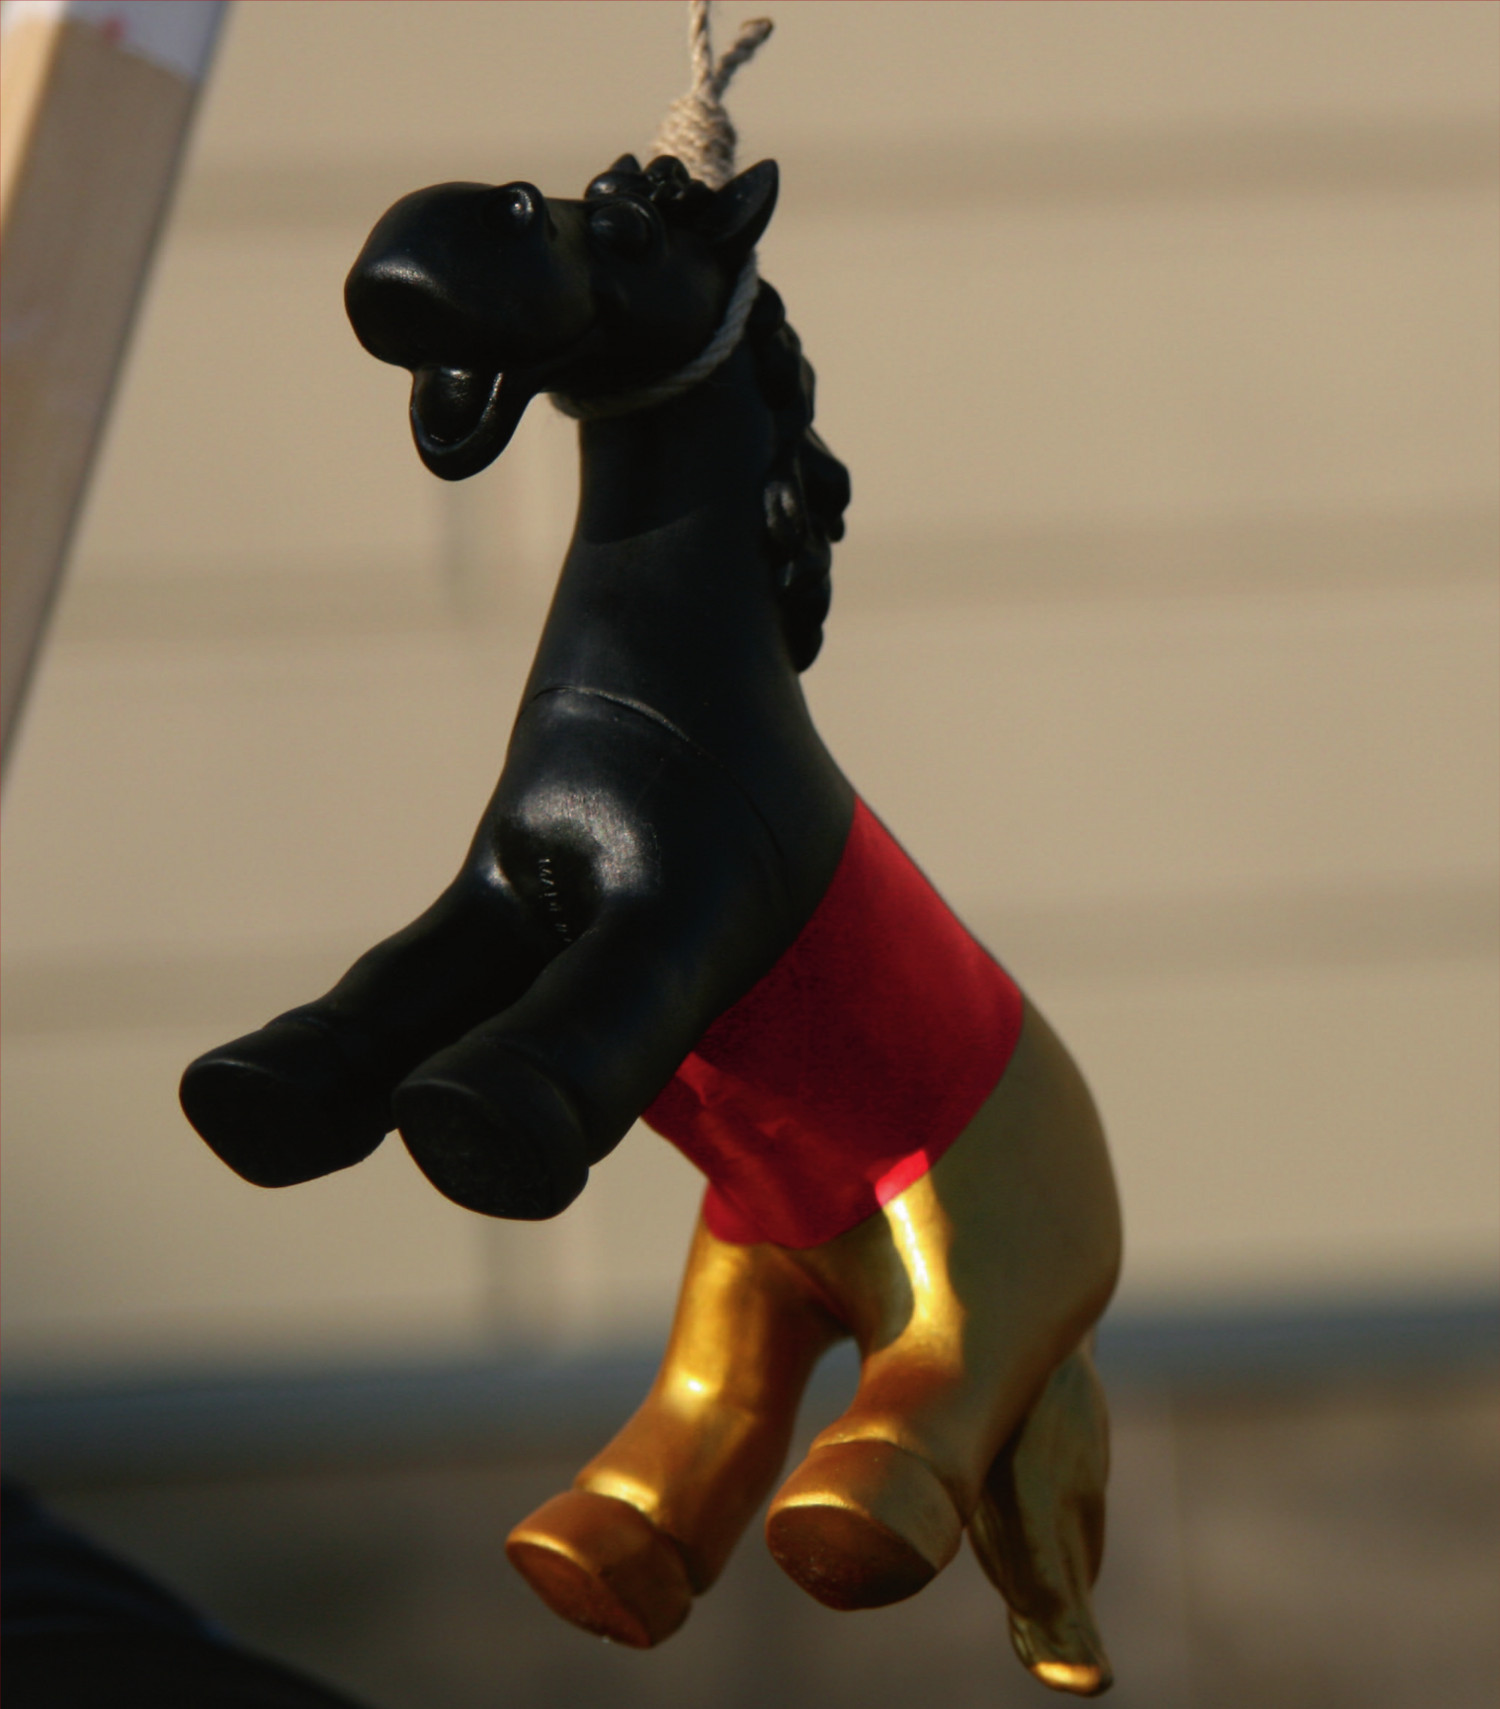
\includegraphics[height=0.7\textheight]{img/trojaner.jpg}
  \end{figure}
\end{frame}

\begin{frame}
    \frametitle{Wer sind wir?}
    \begin{itemize}
      \item<1-> Chaos Computer Club Dresden (\url{http://c3d2.de})
          \note{}
      \item<2-> Datenspuren (\url{http://datenspuren.de})
      \item<3-> Podcasts (\url{http://pentamedia.de})
      \item<4-> Chaos macht Schule
        \begin{itemize}
          \item<2-> \url{http://ccc.de/schule}
          \item<2-> \url{http://c3d2.de/schule.html}
        \end{itemize}
    \end{itemize}
\end{frame}

\begin{frame}
  \frametitle{Soziale Netzwerke}
  \begin{itemize}
    \item Wer ist in welchem sozialen Netzwerk?
      \begin{itemize}
        \item SchülerVZ
        \item SchülerCC
        \item Facebook
        \item Google+
        \item ICQ/MSN/Jabber
        \item Flickr
        \item Last.fm / Jamendo
        \item Youtube
        \item weitere?
      \end{itemize}
  \end{itemize}
\end{frame}

\section{Geschäftsmodelle}
\subsection{}

\begin{frame}
  \frametitle{Geschäftsmodell?}
  \begin{itemize}
    \item<2-> Karstadt
    \item<3-> Amazon
    \item<4-> Ebay
    \item<5-> Facebook
  \end{itemize}
\end{frame}

\begin{frame}
  \frametitle{Einnahmen von Facebook}
  \begin{itemize}
    \item<2-> 82\% Einnahmen aus Werbung
    \item<3-> 30\% Anteil an "`Facebook-Einkäufen"'
    \item<4-> durchschnittlich 1€/Profil
    \item<5-> "`Poweruser"'-Profile deutlich mehr
    \item<6-> => Mehr Werbegewinn durch personalisierte Werbung
  \end{itemize}
\end{frame}

\begin{frame}
  \frametitle{JIM Studie}
  \begin{figure}
    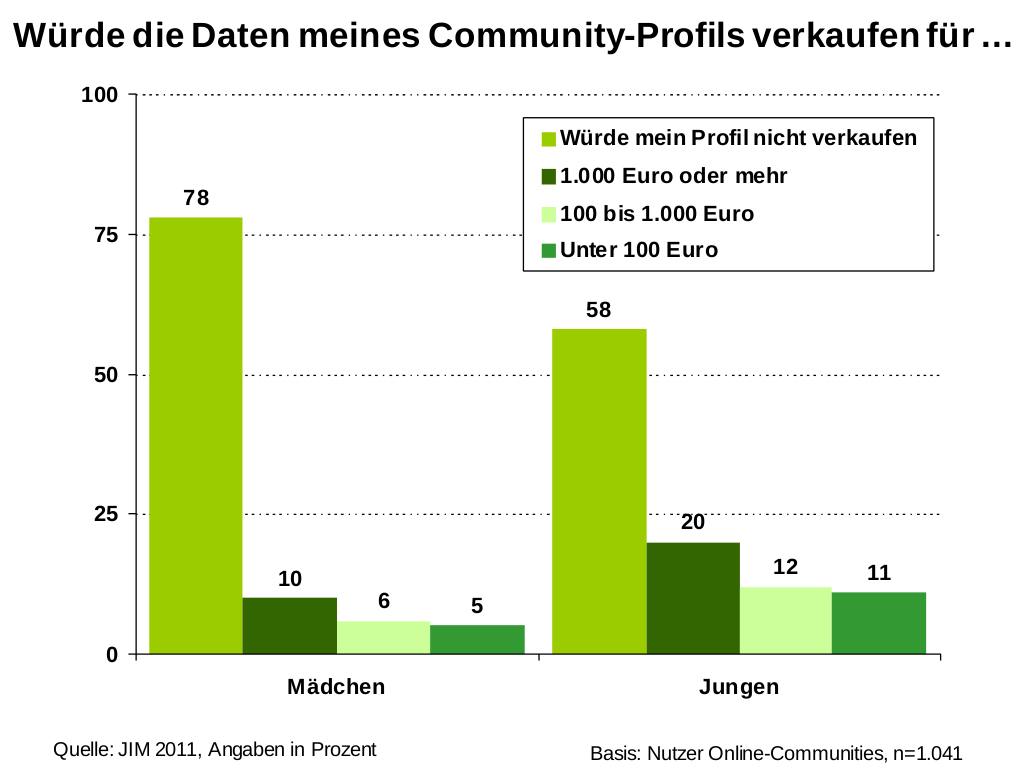
\includegraphics[height=0.7\textheight]{img/jim_verkaufen.png}
  \end{figure}
\end{frame}

\begin{frame}
  \frametitle{Kunde oder Produkt?}
  \begin{figure}
    
\includegraphics[height=0.7\textheight]{img/business_pigs.jpg}
  \end{figure}
\end{frame}

\section{Gefahren}
\subsection{}

\begin{frame}
  \frametitle{You are what you like}
  \begin{itemize}
    \item Geschlecht \textbf{\only<2->{93\%}}
    \item Schwul \textbf{\only<3->{88\%}}
    \item Lesbisch \textbf{\only<4->{75\%}}
    \item Weiß/Dunkelhäutig \textbf{\only<5->{95\%}}
    \item Alkohol \textbf{\only<6->{70\%}}
    \item Rauchen \textbf{\only<7->{73\%}}
  \end{itemize}
\end{frame}

\begin{frame}
  \frametitle{We know what you're doing}
  \begin{center} \Large
   http://www.weknowwhatyouredoing.com/
  \end{center}
\end{frame}

\begin{frame}
  \frametitle{Wen interessierts?}
  \begin{figure}
    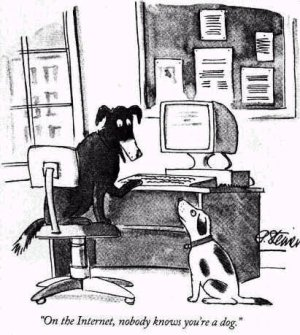
\includegraphics[height=0.7\textheight]{img/internet_dog.jpg}
    \license[http://en.wikipedia.org/wiki/File:Internet\_dog.jpg]{\copyright Image from New Yorker cartoon by Peter Steiner.}
  \end{figure}
\end{frame}

\begin{frame}
  \frametitle{Identität}
  \begin{center} \Large
    Identitätsklau - aus Sicht des Angreifers
  \end{center}
\end{frame}

\begin{frame}
  \frametitle{Personalisiertes Web}
  \begin{center} \Large
     http://howsecureismypassword.net/
  \end{center}
\end{frame}

\begin{frame}
  \frametitle{Personalisiertes Web}
  \begin{itemize}
    \item Passwortsicherheit 
      \begin{itemize}
        \item (nCuAj.§Tsm!f
        \item IchLiebeDich
        \item .§)=")=`
        \item 123456
        \item alkmgfksjr
        \item Mks?o/.u,ePsw!
      \end{itemize}
  \end{itemize}
\end{frame}

\section{Datenschutz}
\subsection{}

\begin{frame}
  \frametitle{Datenschutz - gegenüber wem?}
    \begin{itemize}
      \item<2-> Eltern
      \item<3-> Lehrern
      \item<4-> Freunden
      \item<5-> Unternehmen / Organisationen
      \item<6-> Staat
    \end{itemize}
\end{frame}

\begin{frame}
  \frametitle{Fremde Daten}
  \begin{itemize}
    \item Datenschutz anderer Personen respektieren:
      \begin{itemize}
        \item<2->Bilder taggen
        \item<3->Emailadressen importieren
        \item<4->Angeben, mit wem man etwas unternimmt
      \end{itemize}
  \end{itemize}
\end{frame}

\begin{frame}
  \frametitle{Eigene Daten}
    \begin{itemize}
      \item<2->Moderation von Posts
      \item<3->Freunde auf Fehlverhalten hinweisen
      \item<4->Aufpassen was und wieviel man preisgiebt
      \item<5->Sich bewusst machen, wer was sehen kann
    \end{itemize}
\end{frame}

\begin{frame}
  \frametitle{Posts}
  \begin{itemize}
    \item Wem sollte man preisgeben/posten (und was eher nicht)?
      \begin{itemize}
        \item<2-> "`Roadkill"' von Entertainment for the Braindead ist ein cooles Album
        \item<3-> Jan Müller geht am Donnerstag, den 07.06.2012 zum Poetry Slam in der Scheune
        \item<4-> Ich bin heut' echt gut drauf!
        \item<5-> Ute Meyer war mit Carolin Wittich und Frederik Ulm am Samstag abend im Schillergarten Fußball gucken und ist danach mit Michael Müller nach Hause gefahren
        \item<6-> Meine Lehrerin ist voll doof!
      \end{itemize}
  \end{itemize}
\end{frame}

\begin{frame}
  \frametitle{Pseudonymität}
  \begin{center} \Large
    Pseudonymität
  \end{center}
\end{frame}

\section{Fazit}
\subsection{}

\begin{frame}
  \frametitle{Zusammenfassung}
  \begin{itemize}
    \item Das Internet vergisst nichts
    \item Bewusste Nutzung sozialer Netzwerke
    \item Deine korrekten Daten gehen niemand etwas an
  \end{itemize}
\end{frame}

\end{document}
